\documentclass{InsightArticle}

\usepackage[dvips]{graphicx}
\usepackage{color}
\usepackage{listings}

\definecolor{listcomment}{rgb}{0.0,0.5,0.0}
\definecolor{listkeyword}{rgb}{0.0,0.0,0.5}
\definecolor{listnumbers}{gray}{0.65}
\definecolor{listlightgray}{gray}{0.955}
\definecolor{listwhite}{gray}{1.0}


%%%%%%%%%%%%%%%%%%%%%%%%%%%%%%%%%%%%%%%%%%%%%%%%%%%%%%%%%%%%%%%%%%
%
%  hyperref should be the last package to be loaded.
%
%%%%%%%%%%%%%%%%%%%%%%%%%%%%%%%%%%%%%%%%%%%%%%%%%%%%%%%%%%%%%%%%%%
\usepackage[dvips,
bookmarks,
bookmarksopen,
backref,
colorlinks,linkcolor={blue},citecolor={blue},urlcolor={blue},
]{hyperref}


\title{Principal Components Analysis of\\ Scalar, Vector, and Mesh Vertex Data}


% 
% NOTE: This is the last number of the "handle" URL that 
% The Insight Journal assigns to your paper as part of the
% submission process. Please replace the number "XXXX" with
% the actual handle number that you get assigned.
%
\newcommand{\IJhandlerIDnumber}{XXXX}

\lstset{frame = tb,
       framerule = 0.25pt,
       float,
       fontadjust,
       backgroundcolor={\color{listlightgray}},
       basicstyle = {\ttfamily\footnotesize},
       keywordstyle = {\ttfamily\color{listkeyword}\textbf},
       identifierstyle = {\ttfamily},
       commentstyle = {\ttfamily\color{listcomment}\textit},
       stringstyle = {\ttfamily},
       showstringspaces = false,
       showtabs = false,
       numbers = left,
       numbersep = 6pt,
       numberstyle={\ttfamily\color{listnumbers}},
       tabsize = 2,
       language=[ANSI]C++,
       floatplacement=!h
       }



\release{1.00}

\author{Michael Bowers$^{1}$, Laurent Younes$^{1}$}
\authoraddress{$^{1}$Johns Hopkins University, Baltimore, MD}

\begin{document}


%
% Add hyperlink to the web location and license of the paper.
% The argument of this command is the handler identifier given
% by the Insight Journal to this paper.
% 
\IJhandlefooter{\IJhandlerIDnumber}


\ifpdf
\else
   %
   % Commands for including Graphics when using latex
   % 
   \DeclareGraphicsExtensions{.eps,.jpg,.gif,.tiff,.bmp,.png}
   \DeclareGraphicsRule{.jpg}{eps}{.jpg.bb}{`convert #1 eps:-}
   \DeclareGraphicsRule{.gif}{eps}{.gif.bb}{`convert #1 eps:-}
   \DeclareGraphicsRule{.tiff}{eps}{.tiff.bb}{`convert #1 eps:-}
   \DeclareGraphicsRule{.bmp}{eps}{.bmp.bb}{`convert #1 eps:-}
   \DeclareGraphicsRule{.png}{eps}{.png.bb}{`convert #1 eps:-}
\fi


\maketitle


\ifhtml
\chapter*{Front Matter\label{front}}
\fi


\begin{abstract}
\noindent
This document describes a contribution to the Insight Toolkit intended to
support the analysis of the principal components of data sets, optionally
point data associated with the vertices of a mesh.

This paper is accompanied with the source code, input data, parameters and
output data that we used for validating the implementation described in this
paper.  This adheres to the fundamental principle that scientific publications
must facilitate \textbf{reproducibility} of the reported results.
\end{abstract}

\tableofcontents

\section{Introduction}

Principal Components Analysis (PCA) is a linear transformation created from
sets of measurements to produce a new coordinate system such that the greatest
variance by any projection of the data comes to lie on the first coordinate,
the second greatest on the second coordinate and so on. 

This paper describes a class itk::VectorFieldPCA, an implementation of standard
PCA algorithms for use on
scalar or vector data sets.  Kernel PCA is implemented in this class as well,
where the data sets are scalar or vector valued functions assigned at each of
the points in a \code{PointSet}.  A Gaussian Distance Kernel class is provided
with the PCA class.

This contribution is part of a shape analysis software pipeline created
at Johns Hopkins.  PCA will be used to develop a set of
basis vectors for use with Gaussian Random Field analysis.  The output of PCA
will be analyzed for significance with various statistical methods such as
t-tests built upon the built-in statistical capabilities of ITK.


\section{Template Parameters}

This class is templated over the types of the vector valued functions,
the output data types, and optionally the point set type.  An optional kernel
function type parameter defaults to \code{itk::KernelFunction}.

\section{Inputs}

Input to the class consists of sets of scalar or vector valued data.
The user can set an optional kernel
function to invoke Kernel PCA, and a \code{itk::PointSet} for
kernel operations.  

\section{Outputs}

\begin{itemize}
\item Average of the vector/scalar measurements over all the data sets
\item The eigenvalues of the Principal Components Analysis
\item The set of basis vectors of the data set
\item The projection of the basis onto the vector field set, or any vector set
specified in a call to \code{Projection()}.
\end{itemize}

\section{How to Build}

This contribution includes

\begin{itemize}
\item Source code for the PCA function
\item Tests for the code
\item Test data and output
\end{itemize}

\subsection{Building Executables and Tests}

In order to build the whole, it is enough to configure the directory with
CMake. As usual, an out-of-source build is the recommended method.

In a Linux environment it should be enough to do the following:

\begin{itemize}
\item \code{ccmake  SOURCE\_DIRECTORY}
\item \code{make}
\item \code{ctest}
\end{itemize}

Where SOURCE\_DIRECTORY is the directory where you have expanded the source
code that accompanies this paper.

You will be required to provide the directory where you built or installed ITK.

\begin{itemize}
\item \code{ITK\_DIR}
\end{itemize}

This will configure the project, build the executables, and run the tests and
examples. 


\subsection{Building this Report}

In order to build this report you can do

\begin{itemize}
\item \code{ccmake SOURCE\_DIRECTORY}
\item Turn ON the CMake variables
\begin{itemize}
\item \code{GENERATE\_REPORTS}
\end{itemize}
\item \code{make}
\end{itemize}

This should produce a PDF file in the binary directory, under the subdirectory
\code{Documents/Report001}.

\section{PCA Test Code}

The source code used to test this function provides a good example of its
use.  The scalar PCA test operates on a set of scalar defined functions in
the standard way.  The vector kernel test uses the Gaussian distance kernel
that comes with the class, so a vtkPolyData mesh file is input, as well as
a list of text files containing vector values functions defined at every
vertex in the mesh.

After the PCA calculation, the outputs are available and the test programs
write them out as text data.

The source code presented in this section can be found in the \code{Testing}
directory under the filenames

\begin{itemize}
\item \code{itkScalarPCATest.cxx}

\begin{verbatim}USAGE: itkScalarPCATest [OPTIONS] <outputName> <vectorFieldSetFile>
    -h --help : print this message
    -c --pcaCount : number of principal components to calculate (def = 3)
\end{verbatim}

\item \code{itkVectorKernelPCATest.cxx}

\begin{verbatim}USAGE: itkVectorKernelPCATest [OPTIONS] <vtkMeshFile> <outputName> <vectorFieldSetFile>
    -h --help : print this message
    -c --pcaCount : number of principal components to calculate (def = 3)
    -s --kernelSigma : KernelSigma (def = 6.25)
\end{verbatim}
\end{itemize}

\subsection{Results}

Figure~\ref{fig:HippocampusMomentaAverages} shows the averages for the vector
valued inputs to the test program

\begin{verbatim}itkVectorKernelPCATest -c 5 -s 6.75 -c 5 -s 6.75
    PCATestSurface.vtk vectorPcaOutput
    alpha0_01 alpha0_02 alpha0_03 alpha0_04 alpha0_05
    alpha0_06 alpha0_07 alpha0_08 alpha0_09
    alpha0_10 alpha0_11 alpha0_12 alpha0_13 alpha0_14
    alpha0_15 alpha0_16 alpha0_17 alpha0_18 alpha0_19
    alpha0_20 alpha0_21 alpha0_22 alpha0_23 alpha0_24
    alpha0_25 alpha0_26 alpha0_27 alpha0_28 alpha0_29
    alpha0_30 alpha0_31 alpha0_32 alpha0_33 alpha0_34
    alpha0_35 alpha0_36 alpha0_37 alpha0_38 alpha0_39
\end{verbatim}

The PCATestSurface.vtk input file template altas of a hippocampus surface.  The alpha files
contain the initial momenta vectors at each vertex determined during the calculation of a
deformation between a template and a set of target hippocampus surfaces.
The averages over all the target momenta are displayed in CAWorks, a JHU Center for
Imaging Science Paraview-based application.

\begin{figure}
\center
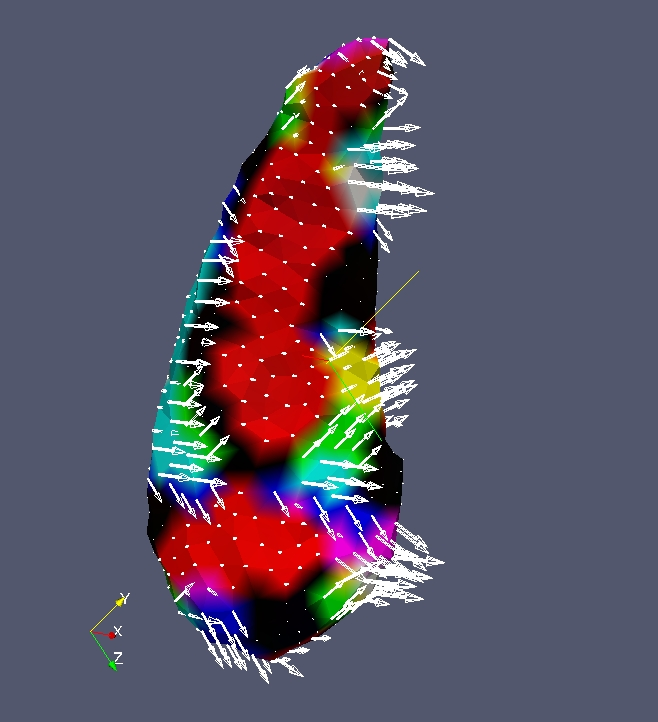
\includegraphics[width=0.8\textwidth]{AveragedMomentumsPREDICT.jpg}
\itkcaption[Hippocampus Momenta Averages]{Momenta averages on a triangulated hippocampus surface.}
\label{fig:HippocampusMomentaAverages}
\end{figure}

\section{Acknowledgements}

Funding for development provided by NIH grants (R01-EB008171-01A1 
and P41-RR015241).

%%%%%%%%%%%%%%%%%%%%%%%%%%%%%%%%%%%%%%%%%
%
%  Insert the bibliography using BibTeX
%
%%%%%%%%%%%%%%%%%%%%%%%%%%%%%%%%%%%%%%%%%

\bibliographystyle{plain}
\bibliography{InsightJournal}

\end{document}
